\documentclass[10pt,twocolumn]{article}
\usepackage[margin=1.8cm]{geometry}
\usepackage{amsmath,amssymb,tcolorbox,float,pgfplots}
\usepackage{minted}
\setminted{fontsize=\scriptsize, bgcolor=gray!5, frame=single, framesep=3mm}
\usepackage{titlesec}
\titleformat{\section}{\large\bfseries}{\thesection}{0.5em}{}
\setlength{\columnsep}{0.6cm}
\pgfplotsset{compat=1.18}

\begin{document}

\begin{center}
{\LARGE \textbf{Work \#18}}\\[4pt]
\textbf{David Fajardo Ríos}\\[8pt]
{\small Analytic Geometry – Tangent Lines and Circles}
\end{center}

\smallskip

% ======================================================
\section*{(i) Tangent Line to the Circle}

\begin{tcolorbox}
Find the equation of the tangent line to the circle
\[
x^{2}+y^{2}-4x+6y-12=0
\]
at the point $(5,1)$.
\end{tcolorbox}

Completing squares:
\[
x^{2}-4x+y^{2}+6y=12 \Rightarrow (x-2)^{2}-4+(y+3)^{2}-9=12,
\]
\[
(x-2)^{2}+(y+3)^{2}=25.
\]
Center \(C(2,-3)\), radius \(r=5.\)

Slope of the radius:
\[
m_r = \frac{1-(-3)}{5-2} = \frac{4}{3}.
\]
Tangent’s slope \(m_t = -\frac{3}{4}\).
\[
y-1 = -\tfrac{3}{4}(x-5) \Rightarrow 3x + 4y - 19 = 0.
\]
\[
\boxed{3x + 4y - 19 = 0.}
\]

\begin{center}
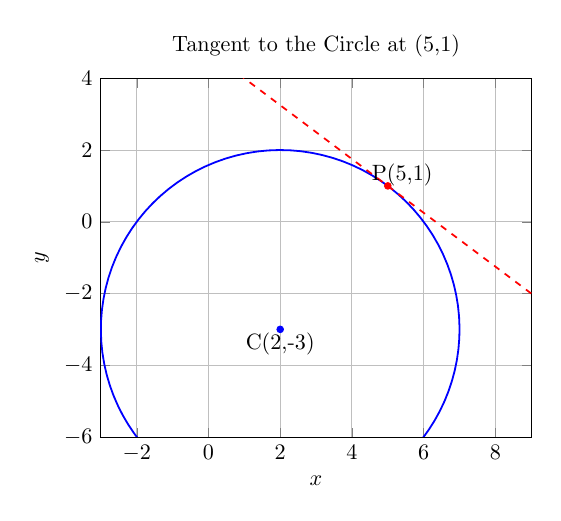
\begin{tikzpicture}[scale=0.8]
\begin{axis}[
    axis equal,
    xmin=-3, xmax=9,
    ymin=-6, ymax=4,
    grid=both,
    xlabel=$x$, ylabel=$y$,
    title={Tangent to the Circle at (5,1)}
]
\addplot [domain=-3:9, samples=200, thick, blue] 
    ({2 + 5*cos(deg(x))}, {-3 + 5*sin(deg(x))});
\addplot [domain=-3:9, samples=2, red, thick, dashed]
    {(-3/4)*(x - 5) + 1};
\addplot [only marks, mark=*, mark size=1.5pt, color=blue] coordinates {(2,-3)};
\addplot [only marks, mark=*, mark size=1.5pt, color=red] coordinates {(5,1)};
\node at (axis cs:2,-3.4) {C(2,-3)};
\node at (axis cs:5.4,1.3) {P(5,1)};
\end{axis}
\end{tikzpicture}
\end{center}

\subsubsection*{Python Code}
\begin{minted}{python}
import numpy as np
import matplotlib.pyplot as plt

theta = np.linspace(0, 2*np.pi, 400)
x = 2 + 5*np.cos(theta)
y = -3 + 5*np.sin(theta)

x_line = np.linspace(-2, 8, 100)
y_line = (-3/4)*(x_line - 5) + 1

plt.plot(x, y, label='Circle')
plt.plot(x_line, y_line, 'r--', label='Tangent')
plt.scatter([2,5], [-3,1], color=['blue','red'])
plt.legend(); plt.axis('equal')
plt.title('Tangent at (5,1)')
plt.show()
\end{minted}

% ======================================================
\section*{(ii) Circle through Three Points}

\begin{tcolorbox}
Find the equation of the circle passing through
$(2,-1)$, $(0,2)$, and $(1,1)$.
\end{tcolorbox}

General form:
\[
x^{2}+y^{2}+Dx+Ey+F=0.
\]
Substitute points and solve:
\[
D=7,\quad E=5,\quad F=-14.
\]
Equation:
\[
\boxed{x^{2}+y^{2}+7x+5y-14=0.}
\]
Center \(C(-\tfrac{7}{2},-\tfrac{5}{2})\),
radius \(r=\tfrac{\sqrt{130}}{2}.\)

\begin{center}
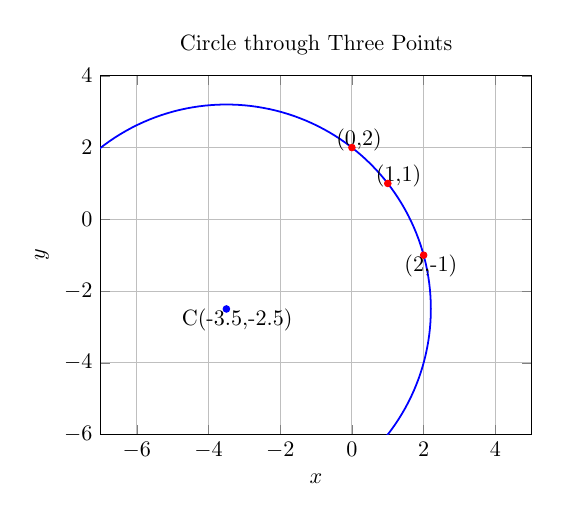
\begin{tikzpicture}[scale=0.8]
\begin{axis}[
    axis equal,
    xmin=-6, xmax=4,
    ymin=-6, ymax=4,
    grid=both,
    xlabel=$x$, ylabel=$y$,
    title={Circle through Three Points}
]
\addplot [domain=0:2*pi, samples=200, thick, blue, variable=\t]
    ({-3.5 + sqrt(65/2)*cos(deg(\t))},
     {-2.5 + sqrt(65/2)*sin(deg(\t))});
\addplot [only marks, mark=*, mark size=1.5pt, color=red]
    coordinates {(2,-1) (0,2) (1,1)};
\addplot [only marks, mark=*, mark size=1.5pt, color=blue]
    coordinates {(-3.5,-2.5)};
\node at (axis cs:-3.2,-2.8) {C(-3.5,-2.5)};
\node at (axis cs:2.2,-1.3) {(2,-1)};
\node at (axis cs:0.2,2.2) {(0,2)};
\node at (axis cs:1.3,1.2) {(1,1)};
\end{axis}
\end{tikzpicture}
\end{center}

\subsubsection*{Python Code}
\begin{minted}{python}
import numpy as np
import matplotlib.pyplot as plt

points = np.array([[2,-1],[0,2],[1,1]])
cx, cy = -3.5, -2.5
r = np.sqrt(65/2)
theta = np.linspace(0, 2*np.pi, 400)
x = cx + r*np.cos(theta)
y = cy + r*np.sin(theta)

plt.plot(x, y, label='Circle')
plt.scatter(points[:,0], points[:,1], color='red')
plt.scatter(cx, cy, color='blue')
plt.legend(); plt.axis('equal')
plt.title('Circle through three points')
plt.show()
\end{minted}

% ======================================================
\section*{(iii) Tangent Condition for the Line}

\begin{tcolorbox}
Find all $k$ values such that
\[
3y - kx = 6
\]
is tangent to
\[
x^{2} - 2x + y^{2} = 3.
\]
\end{tcolorbox}

Completing squares:
\[
(x-1)^{2} + y^{2} = 4.
\]
Center \(C(1,0)\), radius \(r=2.\)

Distance from center to line:
\[
\frac{|k+6|}{\sqrt{k^{2}+9}} = 2
\Rightarrow (k+6)^{2} = 4(k^{2}+9)
\Rightarrow 3k^{2}-12k=0
\Rightarrow \boxed{k=0,\,4.}
\]

\begin{center}
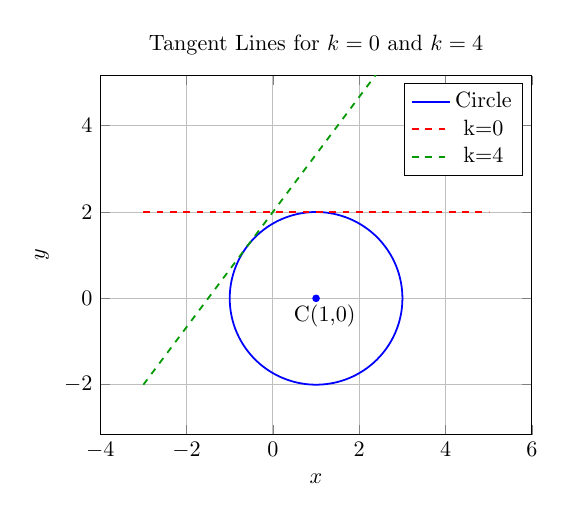
\begin{tikzpicture}[scale=0.8]
\begin{axis}[
    axis equal,
    xmin=-4, xmax=6,
    ymin=-3, ymax=5,
    grid=both,
    xlabel=$x$, ylabel=$y$,
    title={Tangent Lines for $k=0$ and $k=4$}
]
\addplot [domain=0:2*pi, samples=200, thick, blue, variable=\t]
    ({1 + 2*cos(deg(\t))}, {0 + 2*sin(deg(\t))});
\addplot [domain=-3:5, samples=2, red, dashed, thick] {2};
\addplot [domain=-3:5, samples=2, green!60!black, dashed, thick] {(4/3)*x + 2};
\addplot [only marks, mark=*, mark size=1.5pt, color=blue] coordinates {(1,0)};
\node at (axis cs:1.2,-0.4) {C(1,0)};
\legend{Circle, k=0, k=4}
\end{axis}
\end{tikzpicture}
\end{center}

\subsubsection*{Python Code}
\begin{minted}{python}
import numpy as np
import matplotlib.pyplot as plt

theta = np.linspace(0, 2*np.pi, 400)
x = 1 + 2*np.cos(theta)
y = 2*np.sin(theta)

x_line = np.linspace(-3, 5, 100)
plt.plot(x, y, label='Circle')
plt.plot(x_line, np.ones_like(x_line)*2, 'r--', label='k=0')
plt.plot(x_line, (4/3)*x_line + 2, 'g--', label='k=4')
plt.scatter([1], [0], color='blue')
plt.legend(); plt.axis('equal')
plt.title('Tangent lines for k=0 and k=4')
plt.show()
\end{minted}
\section*{2. Region plots of inequalities}

\begin{tcolorbox}
Draw the set of all points that satisfy each inequality:
\begin{enumerate}
\item[(a)] $(x-1)^{2}+(y+5)^{2}\le25$
\item[(b)] $1\le x^{2}+y^{2}\le4$
\item[(c)] $x^{2}+y^{2}>2y$
\item[(d)] $x>y^{2}$
\item[(e)] $y<x^{2}+1$
\end{enumerate}
\end{tcolorbox}

% ---- (a)
\subsection*{(a) $(x-1)^{2}+(y+5)^{2}\le25$}
Circle centered at $(1,-5)$ with radius $5$.

\begin{center}
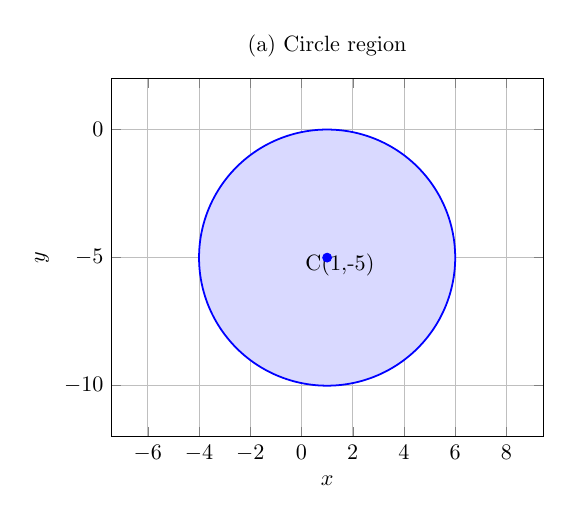
\begin{tikzpicture}[scale=0.8]
\begin{axis}[
    axis equal,
    xmin=-6, xmax=8, ymin=-12, ymax=2,
    grid=both, xlabel=$x$, ylabel=$y$,
    title={(a) Circle region}
]
\addplot [domain=0:2*pi, samples=200, fill=blue!15, draw=blue, thick, variable=\t]
    ({1 + 5*cos(deg(\t))}, {-5 + 5*sin(deg(\t))});
\addplot [only marks, mark=*, color=blue] coordinates {(1,-5)};
\node at (axis cs:1.5,-5.3) {C(1,-5)};
\end{axis}
\end{tikzpicture}
\end{center}

\subsubsection*{Python Code}
\begin{minted}{python}
import numpy as np, matplotlib.pyplot as plt
theta = np.linspace(0, 2*np.pi, 400)
x, y = 1 + 5*np.cos(theta), -5 + 5*np.sin(theta)
plt.fill(x, y, color='skyblue', alpha=0.4)
plt.scatter(1, -5, color='blue')
plt.axis('equal'); plt.title('(x-1)^2 + (y+5)^2 <= 25')
plt.show()
\end{minted}

% ---- (b)
\subsection*{(b) $1 \le x^{2}+y^{2} \le 4$}
Annulus between two concentric circles.

\begin{center}
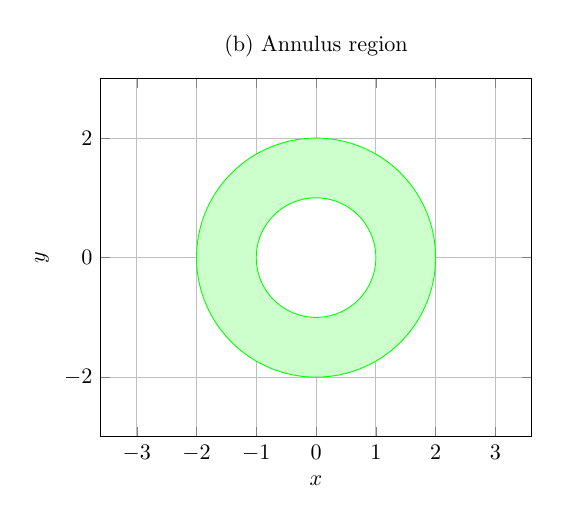
\begin{tikzpicture}[scale=0.8]
\begin{axis}[
    axis equal,
    xmin=-3, xmax=3, ymin=-3, ymax=3,
    grid=both, xlabel=$x$, ylabel=$y$,
    title={(b) Annulus region}
]
% Outer circle
\addplot [domain=0:2*pi, samples=200, fill=green!20, draw=green, variable=\t]
    ({2*cos(deg(\t))}, {2*sin(deg(\t))});
% Inner circle (white fill to create ring)
\addplot [domain=0:2*pi, samples=200, fill=white, draw=green, variable=\t]
    ({1*cos(deg(\t))}, {1*sin(deg(\t))});
\end{axis}
\end{tikzpicture}
\end{center}

\subsubsection*{Python Code}
\begin{minted}{python}
theta = np.linspace(0, 2*np.pi, 400)
xo, yo = 2*np.cos(theta), 2*np.sin(theta)
xi, yi = np.cos(theta), np.sin(theta)
plt.fill(xo, yo, color='lightgreen', alpha=0.5)
plt.fill(xi, yi, color='white')
plt.axis('equal'); plt.title('1 <= x^2 + y^2 <= 4')
plt.show()
\end{minted}

% ---- (c)
\subsection*{(c) $x^{2}+y^{2}>2y$}
Equivalent to $(x)^{2}+(y-1)^{2}>1$: exterior of a circle centered at $(0,1)$.

\begin{center}
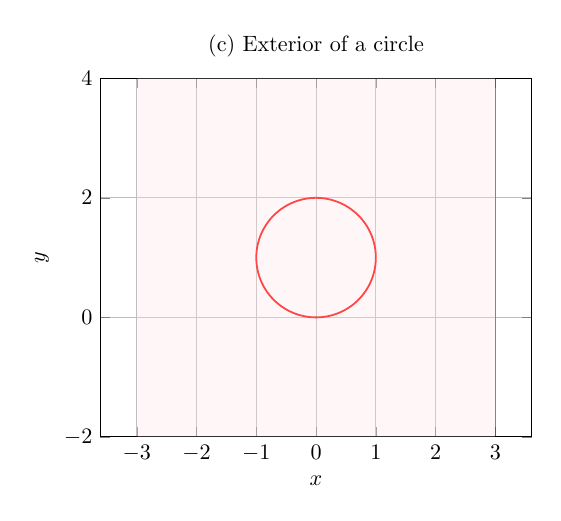
\begin{tikzpicture}[scale=0.8]
\begin{axis}[
    axis equal,
    xmin=-3, xmax=3, ymin=-2, ymax=4,
    grid=both, xlabel=$x$, ylabel=$y$,
    title={(c) Exterior of a circle}
]
% Circle boundary
\addplot [domain=0:2*pi, samples=200, draw=red, thick, variable=\t]
    ({cos(deg(\t))}, {1 + sin(deg(\t))});
% Shaded region outside (approx)
\addplot [fill=red!10, opacity=0.3] coordinates {(-3,-2) (3,-2) (3,4) (-3,4)};
\end{axis}
\end{tikzpicture}
\end{center}

\subsubsection*{Python Code}
\begin{minted}{python}
theta = np.linspace(0, 2*np.pi, 400)
x, y = np.cos(theta), 1 + np.sin(theta)
plt.plot(x, y, 'r')
plt.fill_between(x, 4, y, color='mistyrose', alpha=0.4)
plt.axis('equal'); plt.title('x^2 + y^2 > 2y')
plt.show()
\end{minted}

% ---- (d)
\subsection*{(d) $x>y^{2}$}
Region to the right of the parabola $x = y^{2}$.

\begin{center}
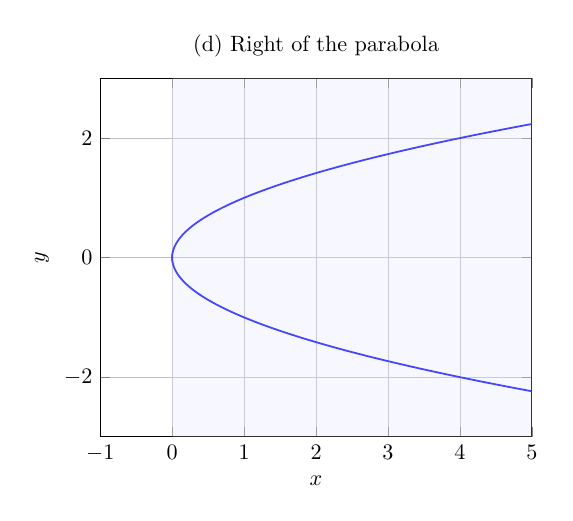
\begin{tikzpicture}[scale=0.8]
\begin{axis}[
    xmin=-1, xmax=5, ymin=-3, ymax=3,
    grid=both, xlabel=$x$, ylabel=$y$,
    title={(d) Right of the parabola}
]
\addplot [domain=-3:3, samples=200, thick, blue] ({x^2}, {x});
\addplot [fill=blue!10, opacity=0.3] coordinates {(0,-3) (5,-3) (5,3) (0,3)};
\end{axis}
\end{tikzpicture}
\end{center}

\subsubsection*{Python Code}
\begin{minted}{python}
y = np.linspace(-3, 3, 400)
x = y**2
plt.plot(x, y, 'b')
plt.fill_betweenx(y, x, 5, color='skyblue', alpha=0.3)
plt.axis('equal'); plt.title('x > y^2')
plt.show()
\end{minted}

% ---- (e)
\subsection*{(e) $y < x^{2}+1$}
Region below the parabola $y = x^{2}+1$.

\begin{center}
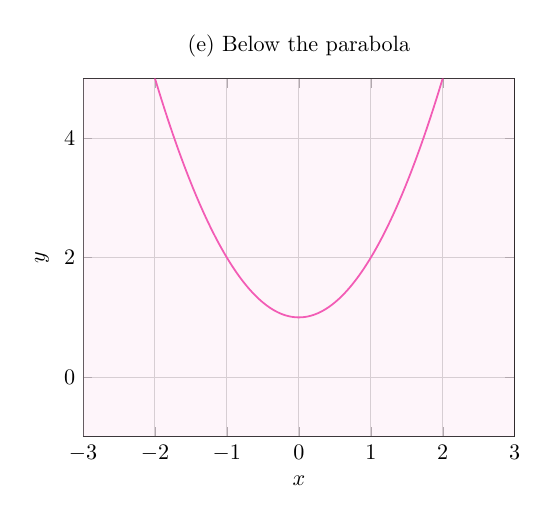
\begin{tikzpicture}[scale=0.8]
\begin{axis}[
    xmin=-3, xmax=3, ymin=-1, ymax=5,
    grid=both, xlabel=$x$, ylabel=$y$,
    title={(e) Below the parabola}
]
\addplot [domain=-3:3, samples=200, thick, magenta] {x^2 + 1};
\addplot [fill=magenta!10, opacity=0.4] coordinates {(-3,-1) (3,-1) (3,5) (-3,5)};
\end{axis}
\end{tikzpicture}
\end{center}

\subsubsection*{Python Code}
\begin{minted}{python}
x = np.linspace(-3, 3, 400)
y = x**2 + 1
plt.plot(x, y, 'm')
plt.fill_between(x, -1, y, color='pink', alpha=0.4)
plt.axis('equal'); plt.title('y < x^2 + 1')
plt.show()
\end{minted}

\end{document}
% Hola mundo
% prueba 2